\documentclass[12pt, a4paper, titlepage]{article}
\usepackage[utf8]{inputenc}
\usepackage[ruled,vlined]{algorithm2e}

\usepackage{amsmath}
\usepackage{hyperref}

\usepackage[a4paper,bindingoffset=0.2in,%
            left=1in,right=1in,top=1in,bottom=1in,%
            footskip=.25in]{geometry}

\usepackage{eso-pic}
\usepackage[]{graphicx}
\AddToShipoutPictureBG*
  {%
    \put(\LenToUnit{.72\paperwidth}, \LenToUnit{.87\paperheight})
      {
\includegraphics[width=50mm,scale=0.5]{logo.jpg}}%
  }
\providecommand{\keywords}[1]
{
  \small	
  \textbf{\textit{Keywords---}} #1
}

\title{
    \textbf{Problème du cercle minimum : Welzl Algorithm}\\
    \begin{large} 
    Conception et Pratique de l'Algorithmique
    \end{large}
    }
\author{Alexandre EM}
\begin{document}
\maketitle

\begin{abstract}
    Étant donne un ensemble de point $P$ dans un plan à 2 dimensions, le cercle minimum couvrant $P$ est le cercle qui englobe l'ensemble de point avec un diamètre minimal et donc la distance maximale de deux points de $P$. Nous allons étudier un algorithme simple qui permettra de calculer le cercle minimal couvrant d'un ensemble fini de points, l'algorithme de Welzl. Cet algorithme récursif va séparer l'ensemble de points en deux sous ensemble: les points qui appartiennent au cercle et ceux qui sont à la bordure du cercle et grâce à ce sous ensemble, calculer le cercle minimum assez rapidement.\\
    
\keywords{Welzl, Géométrie algorithmique, cercle minimum, diamètre}
\end{abstract}
\tableofcontents
\newpage
\section{Introduction}
    Le problème du cercle minimum ou "minimum enclosing circle problem", en anglais est un problème mathématique pour calculer le cercle de rayon minimum couvrant tout un ensemble de points sur un même plan.\\
    Il existe plusieurs applications où la résolution de ce problème dans la vie courante est utile, tel que : Décider de la position d'un établissement qui serait fréquenté, comme une école, hôpital, mairie, etc. afin de minimiser la distance entre l'établissement et les habitants de la ville, région, etc. les plus éloignés. Dans le milieu militaire, cela serait de déterminer le bon endroit où faire atterrir une bombe pour détruire une cible. Le rayon du cercle permettrait de calculer la puissance de l'explosion requise. Connus sous le nom de \textit{Bomb problem}. Dans le milieu du jeu vidéo, cela serait pour détecter la collision d'objets circulaires ou s'en rapprochant, etc.\\
    
    Afin de résoudre ce problème, on peut utiliser un algorithme naïf qui comparerait tous les cercles formés par les points appartenant à l'ensemble de points. Cependant la complexité temporelle de cette algorithme est de $O(n^{4})$ ce qui n'est pas rapide. Il existe différents algorithmes résolvant le problème du cercle minimum plus rapidement. Parmi ceux que l'on a étudié, il y a l'algorithme de Ritter, qui très rapide mais qui est une approximation du cercle minimum, et celui de Welzl qui est le sujet de ce projet.
\section{Définitions, Notations}
\subsection{Notation}
    Dans la suite de ce rapport, nous allons noter :
    \begin{itemize}
        \item $N$, le plan en 2 dimensions dans lequel nous effectuons l'étude
        \item $P$, l'ensemble des points, de taille $n$ appartenant au plan $N$, un point $p \in P$ possède des coordonnées notées $p.x$ et $p.y$
        \item $C$, un cercle appartenant au plan $N$, de rayon $r$ et de centre $c$
    \end{itemize}
    
    \subsection{Définition}

        \subsubsection{Distance entre 2 points}
        Soit $p,q$ deux points avec des coordonnées $x$ et $y$, la distance $d$ de ces deux points est égale à : 
            \begin{equation}\label{eq:distance}
                d = \sqrt{(p.x - q.x)^{2} + (p.y - q.y)^{2}}
            \end{equation}
        \subsubsection{Coordonnées du milieu d'un segment}
        Soit $p,q$ deux points avec des coordonnées $x$ et $y$, le milieu $m$ de [$p,q$] est égal à:
        \begin{equation}
            m = [\frac{p_{1}.x+p_{2}.x}{2}, \frac{p_{1}.y+p_{2}.y}{2}]
        \end{equation}
        \subsubsection{Point appartenant à un cercle}
        Soit $P \in N$, On dit qu'un point $p \in P$ est couvert par un cercle $C$ de rayon $r$ et de centre $c$, si :
        \begin{equation}
            ((p.x - c.x)^{2} + (p.y - c.y)^{2}) \leq r^{2}
        \end{equation}
        \subsubsection{Cercle minimum couvrant}
         Soit $P \in N$, et soit un cercle $C \in N$. On peut donc dire que $C$ est un cercle minimum de $P$ si et seulement si $\forall p \in P,$ \space $p \subset C$ et que son diamètre est plus petit que les diamètres de tous les cercles appartenant à l'ensemble des cercles couvrant les points de $P$.
         
        \subsubsection{Cercle circonscrit}
        Soit {$p_{1}, p_{2}, p_{3} \in P$} non colinéaires, et $d_{1}, d_{2}, d_{3}$, les droites passant par le milieu des segments de chaque pair des points de $P$. Le centre du cercle circonscrit se trouve à l'intersection des droites $d_{1}, d_{2}, d_{3}$.\\
        Soit le milieu $m$ de [$p_{1},p_{2}$] et $n$ celui de [$p_{1},p_{3}$]:
         \begin{equation}
             m=(\frac{p_{1}.x + p_{2}.x}{2}, \frac{p_{1}.y + p_{2}.y}{2}) \;\;\;et\;\;\; n = (\frac{p_{1}.x + p_{3}.x}{2}, \frac{p_{1}.y + p_{3}.y}{2})
         \end{equation}
        et soit $m.y=\alpha_{1}*m.x + \beta_{1}$, l'équation de la droite passant par le point $m$ et perpendiculaire à la droite ($p_{1},p_{2}$) et $n.y=\alpha_{2}*n.x + \beta_{2}$, l'équation de la droite passant par le point $n$ et perpendiculaire à la droite ($p_{1},p_{3}$). On peut en déduire $\alpha et \beta$:
        \begin{equation}
            \alpha_{1} = (\frac{p_{2} - p_{1}.x}{p_{1}.y - p_{2}.y}) \;\;\;et\;\;\; \beta_{1} = m.y - \alpha_{1} \times m.x
        \end{equation}
        Et pareillement pour ceux de $n$. On peut alors déterminer les coordonnées du centre $c$ de $C$, qui est l'intersection des deux droites. 
        \begin{equation}
            c = ( \frac{\beta_{2} - \beta_{1}}{\alpha_{2} - \alpha_{1}} , \alpha_{1} \times c.x + \beta_{1} )
        \end{equation}
        Et le rayon $r$ de $C$ est alors la $distance^{\eqref{eq:distance}}$ entre un point et le centre $c$ que l'on vient de calculer.
        
        \subsubsection{Cas de base}\label{eq:bases}
        Soit $P \in N$, et $C$ le cercle couvrant minimum de $P$
        \begin{enumerate}
            \item si $P = \emptyset$, alors il n'y a pas de cercle couvrant $C$
            \item si $P = \{p\}$, $p$ étant le seul point de $P$, il est donc le centre de $C$ de rayon $0$
            \item si $P = \{p_{1}, p_{2}\}$, alors $C$ est de centre m, le milieu du segment [$p_{1}$, $p_{2}$], de rayon $\frac{d}{2}$, avec $d$, la distance entre $p_{1}$ et $p_{2}$
            \item si $P = \{p_{1}, p_{2}, p_{3}\}$, On effectue pour chaque pair de points, le \textit{cas(3)} et si $\forall p_{i \in \{1,2,3\}},$\space$p_{i} \subset C'$, $C'$ le cercle obtenu précédemment. Sinon $C$ est le cercle circonscrit obtenu par les points de $P$ 
        \end{enumerate}


\section{Algorithme Naïf}
    \subsection{Description}
    Un algorithme naïf est un algorithme qui permet d'obtenir une solution intuitif, correcte sans se préoccuper des problèmes de complexité et essayer d'optimiser. Il servira donc ensuite de base pour en construire un qui sera plus optimal.\\
     L'algorithme naïf de ce problème, consiste tout d'abord de tester tous les cercles crées par 2 points de $P$, de centre de position du milieu du segment de ces deux points et si un cercle $C$ couvre l'intégralité des points de $P$ alors $C$ est un cercle couvrant minimum de l'ensemble $P$. Si aucun cercle couvrant n'est trouvé, alors l'algorithme parcourt tous les points de $P$ et vérifie que le cercle circonscrit formé par 3 points de $P$ couvre tous les points de $P$.\\

    \begin{algorithm}[H]
    \SetAlgoLined
    \KwData{P: Liste des points}
    \KwResult{C: Le cercle couvrant minimum }
    \BlankLine
    \For{$p \in P$}{
      \For{$q \in P$}{
        $C \leftarrow$ cercle de centre $\frac{p+q}{2}$ de diamètre $|pq|$\;
        \If{$C$ couvre tous les points de $P$}{
            retourne $C$\;
        }
      }
    }
    $C$ $\leftarrow$ cercle de rayon infini\;
      \For{$p \in P$}{
        \For{$q \in P$}{
            \For{$r \in P$}{
                $c \leftarrow $ cercle circonscrit de $\{p.q.r\}$\;
                \If{$c$ couvre tous les points de $P$ et $c$ plus petit que $C$}{
                    $C \leftarrow c$\;
                }
            }
        }
      }
    retourne $C$\;
     \caption{Naïf}
    \end{algorithm}
    \subsection{Terminaison et calcul de la complexité de l'algorithme naïf}
    La complexité temporelle de cet algorithme est de l'ordre de $O(n^{4})$, avec $n$ le nombre de points dans $P$,
    \begin{itemize}
        \item Dans la condition de la première double boucle for, l'algorithme parcours tous les points donc $O(n)$ et pareil pour la double boucle for imbriquée qui a donc une complexité totale de $O(n^{3})$
        \item Pareillement pour la condition de la triple boucle, on a donc une complexité totale de la triple boucle de  $O(n^{4})$ 
    \end{itemize}
    On peut en conclure que l'algorithme possède une complexité totale de l'ordre $O(n^{3})+O(n^{4}) = O(n^{4})$

    \subsection{Résultat des tests de l'implémentation}
    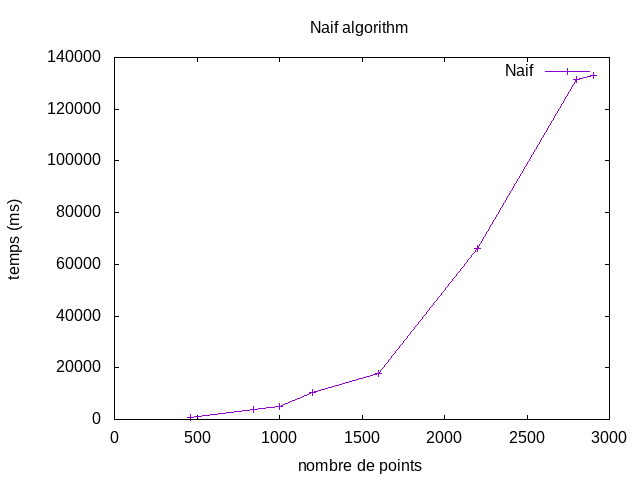
\includegraphics[width=365px,
                     keepaspectratio,]{NaifPoints.png}\\
    Nous remarquons que par l'allure de cette courbe à l'air de correspondre à la complexité de l'algorithme.
    Les test JUnit de l'algorithme Naïf sont situés dans la classe testNaif du package \texttt{test}.\\
    L'algorithme passe les tests des cas de base défini dans la \textit{section 2} du rapport, mais pas pour 1664 instances de test de la base de test de Veroumas. Nous testons qu'un cercle est couvrant minimum lorsque la distance entre le centre du cercle $c$ et tous les points $p \in P$ est inférieur au rayon du cercle. Le nombre de test qui passe est de $\sim740$ instances. Cela peut être du au fait que l'on doit convertir des nombres décimal en entier, ce qui créer des erreurs dans les tests. \\
    
    \begin{center}
    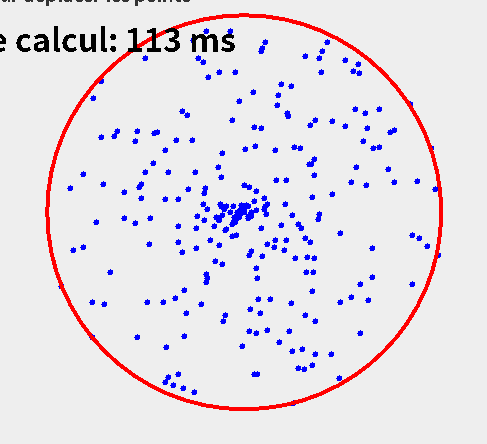
\includegraphics[width=175px,
                     keepaspectratio,]{Screenshot from 2021-01-23 17-10-24.png}
    \end{center}
    
    Nous pouvons voir qu'il existe des points à l'extérieur du cercle, mais qui sont à la frontière de la bordure du cercle, d'où l'invalidité du test unitaire sur certaines instances dans la base de test de Vemouras.
\section{Algorithme de Welzl}
    \newtheorem{lemme}{Lemme}
    \begin{lemme}
        Soit $P$ et $R$ des ensembles finis de points dans un plan, tel que $P \neq \emptyset$ et que $\exists p \in P$
        \begin{enumerate}
            \item Si il existe un cercle contenant $P$ et $R$, dans ses bordures, alors le cercle minimum $b\_md(P, R)$ est bien défini et unique.
            \item Si $p \notin b\_md(P - {p}, R)$, alors le point est inclus dans $R$ et donc dans le cercle minimum $b\_md(P-{p}, R \cup {p}) = b\_md(P, R)$
            \item si le cercle $b\_md(P, R)$ existe, il y a un sous ensemble d'au $max(0, 3-|R|)$ points de P tel que, $b\_md(P, R) = b\_md(S, R)$
        \end{enumerate}
    \end{lemme}
    \subsection{Description}
    L'algorithme de Welzl est donc un algorithme récursif, qui permet de calculer un cercle minimal, en temps linéaire, et qui est basé sur l'algorithme sur le programme linéaire de \textit{Seidel}. Il y a aussi algorithme de \textit{Megiddo}, qui est un algorithme d'élagage de complexité linéaire mais qui est difficile à comprendre et à implémenter par rapport a celui de Welzl.
    L'algorithme de Welzl prend en entrée $P$ la liste de points dans le plan $N$ et R la liste des points qui seront en dehors du cercle et donc initialisé à $\emptyset$.\\
    L'algorithme choisi aléatoirement un point $p \in P$, puis fait un appel récursif afin de trouver un cercle minimum couvrant sans le point $p$. Si ce cercle $C$ existe et que $p$ est inclus dedans alors l'algorithme retourne $C$, sinon on fait un autre appel récursif avec $p$ dans l'ensemble des points situés aux bordures du cercle.\\
    Lorsque l'ensemble $R$ contient \textbf{3 points} ou que $P$ ne contient \textbf{plus de points}, alors l'algorithme passe dans les $cas\; de\; base^{\eqref{eq:bases}}$ et cela renvoie un cercle minimum couvrant de $P$ et $R$, points situés dans la bordure du cercle.\\
    
    \begin{algorithm}[H]
    \SetAlgoLined
    \KwData{$P$: Liste des Points de taille $n$, $R$=$\emptyset$: Liste de Point}
    \KwResult{$C$: Cercle minimum couvrant P}
        $D \leftarrow$ Cercle vide\;
        \eIf{$P = \emptyset$ or $|R| = 3$}{
            $D \leftarrow$ Cas de base appliqué à $R$\;
        }{
            $p \leftarrow$ point aléatoire $\in P$\;
            $D \leftarrow$ Welzl($P - \{p\}, R$)\;
            \If{$D$ défini and $p \notin D$}{
                $D \leftarrow$ Welzl($P - \{p\}, R \cup \{p\}$)\;
            }
        }
        retourne $D$
    \caption{Welzl}
    \end{algorithm}

    \subsection{Terminaison et calcul de la complexité de l'algorithme}
        C'est un algorithme récursif, et la première condition correspond au cas de base, qui sont définis dans la \textit{section 2} du rapport, et qui retourne un cercle. Dans la suite de l'algorithme, il prend un point au hasard et fait un appel récursif à l'algorithme et si la condition de la ligne suivante n'est jamais appelé alors il répète la récursion jusqu'à ce qu'il n'y ait plus de points dans $P$ et on entre dans le cas de base, l'algorithme se termine donc. Si il entre dans la condition mais que dans toutes les récursions $R$ n'a jamais 3 points, $P$ devient vide et alors on retombe dans le même cas précédent et donc dans le cas de base. Et si $R$ contient 3 points, il valide aussi la première condition et c'est le cas de base. L'algorithme se termine bien.\\
        La complexité temporelle de l'algorithme de Welzl est de l'ordre de $O(n)$, avec $n$ le nombre de points dans $P$,
        \begin{itemize}
            \item Les 3 premiers cas de base sont des opérations basiques donc leurs complexités est de l'ordre de $O(1)$, dans le quatrième cas il y a une double boucle for, mais on sait que la taille de $R$ est borné à 3 donc dans le pire des cas, on a une complexité de $O(3^{2})= O(9)$ donc l' appel à la fonction de base est de l'ordre de $O(1)$. 
            \item On parcours tous les points de $P$, qui est de l'ordre de $O(n)$
        \end{itemize}
        On peut donc en conclure que l'algorithme de Welzl possède une complexité temporelle de l'ordre de $O(n)$.\\
        L'algorithme est très rapide mais le nombre de points que l'on peut tester sur machine est très limiter par rapport à la pile d'appels. Il serait donc plus intéressant de l'implémenter itérativement afin de pouvoir faire tourner l'algorithme sur des instances contenant un nombre de points plus important. 
    
    \subsection{Résultat des tests de l'implémentation}
        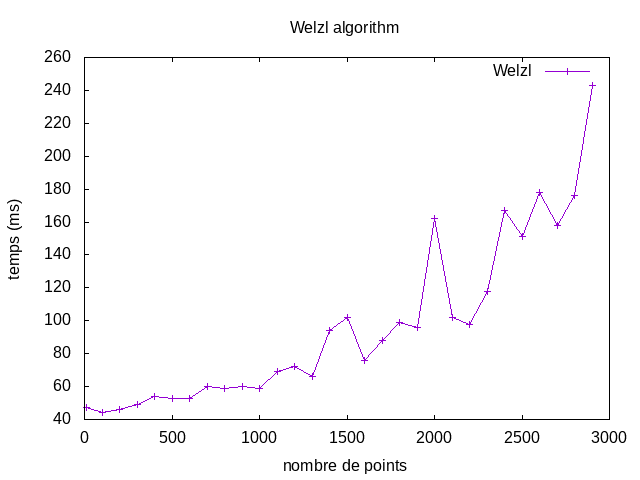
\includegraphics[width=355px,
                        keepaspectratio,]{welzlPoints2.png}\\
        
        Dans cette courbe, nous pouvons remarquer que la courbe a une allure linéaire, même s'il y a des pics a certains endroit, cela peut peut-être dû à la position des points dans le plan.\\
        Les test JUnit de l'algorithme Naïf sont situés dans la classe testWelzl du package \texttt{test}.\\
        \begin{center}
            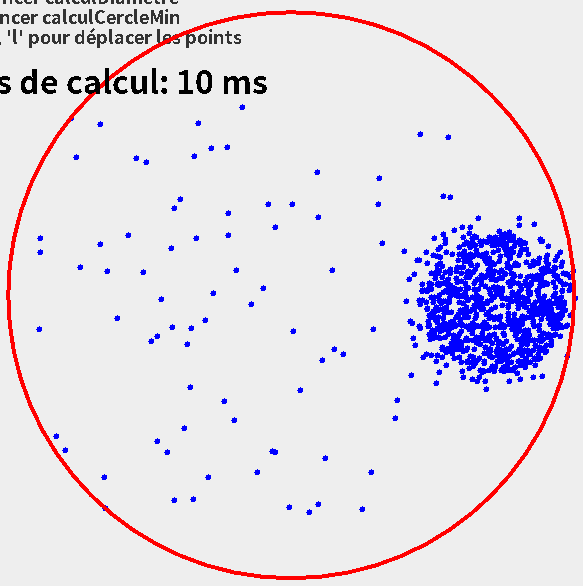
\includegraphics[width=175px, keepaspectratio,]{Screenshot from 2021-01-24 16-35-13.png}
        \end{center}
        Dans le même cas que l'algorithme naïf, les tests valident l'algorithme pour les cas de base, mais ne les valident pas pour les 1664 instances de test de la base de test de Veroumas, en comparant la taille des deux rayons des cercles obtenus pour la même instance. Le nombre de test qui valide l'implémentation est variable car la taille du cercle minimum varie, nous avons environ $710$ instances valides et $\sim800$ lorsque l'on compare les deux cercle obtenu par les 2 algorithmes. Si on regarde la figure au dessus, on peut remarquer que certains points sont à la frontière de la bordure du cercle. Cela peut s'expliquer par la conversion de $double$ en $int$ lors de la création des points du cercle.

\section{Observation}
    Afin d'observer le comportement des deux algorithmes, nous avons testé sur une base de test de \textit{Vemouras} contenant 1664 instances avec un nombre de points fixe de 256. Nous avons écrit un script bash qui permet de générer, de collecter les données nécessaires puis de générer les diagrammes liées avec \textit{Gnuplot}.\\
    Nous avons implémenté les algorithmes, en \textbf{Java} où:
    \begin{itemize}
        \item Point est un Objet Java composé de ses coordonnées $x,y: entier$
        \item Cercle est un Objet composé d'un $centre : Point$ et d'un $rayon: entier$
        \item L'ensemble des points $P$ est une Liste de $Point$
    \end{itemize}
    Et les tests sont effectués sur une machine composé de 4 coeurs et de 8 Go de ram.
    \subsection{Comparaison des rayons des cercles obtenus par les 2 algorithmes}
    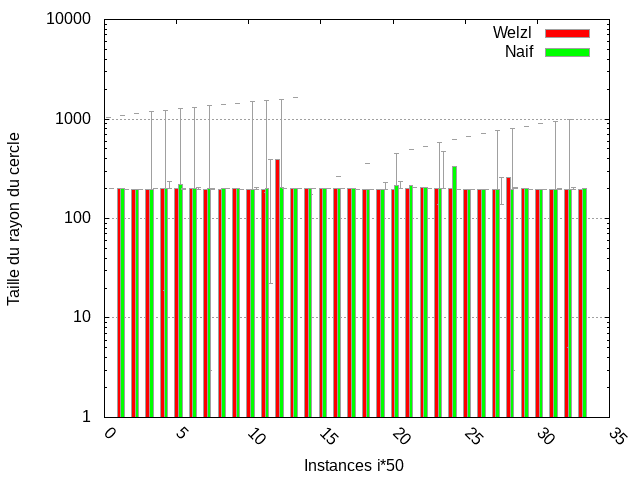
\includegraphics[width=395px,
                     keepaspectratio,]{testResult.png}
    
    Nous avons vérifié l'échelle de validité de l'implémentation de l'algorithme de Welzl en le comparant à l'implémentation de l'algorithme Naïf qui est censé être valide. Pour cela, nous avons testé la taille du rayon du cercle renvoyé pour 1664 instances avec $n=256$ de la base de test de \textit{Varoumas}, sur les deux algorithmes. Étant donné que le diagramme était illisible pour 1664 instances, nous avons pris les données à chaque 50 instances donc la dernière instance dans le diagramme est la numéro $33\times 50 = 1650$\\
    Si on compare la taille du rayon du cercle minimum calculé par les implémentations des deux algorithmes, on remarque qu'il y a peu de différences entres les deux tailles, mais que pour certaines instances, il y a un écart non négligeable des deux rayons et on peut donc dire que pour ces instances, l'algorithme de Welzl n'a pas pu calculer dès la première fois le cercle minimum de $P$. Effectivement, lorsque nous avons testé l'implémentation graphiquement, il y avait des probabilités qu'il ne dessine pas dès la première fois le cercle min \\
    Pour certaines instances, le rayon du cercle calculé par l'algorithme de Welzl est plus petit que celui qui est calculé par le naïf et dans ce cas la nous pensons que la récursion de l'algorithme doit s'être arrêter trop tôt.
    
    \subsection{Comparaison du temps d'exécution des 2 algorithmes sur un même nombre de points }
    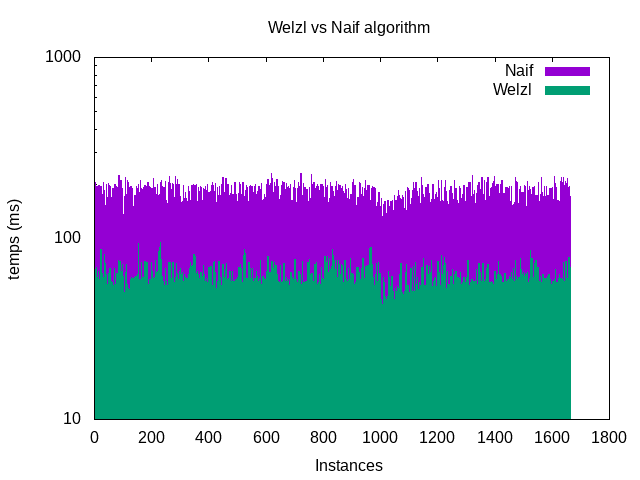
\includegraphics[width=370px,
                     keepaspectratio,]{welzlNaif.png}
    
    Nous avons comparé les deux algorithmes pour les 1664 instances de Vemouras pour chaque instances et récuperer le diagramme à l'échelle logarithmique obtenu grâce au données collectés. Nous pouvons remarquer que la forme des deux histogramme sont presque identiques. Par la variation du temps d'exécution, nous remarquons aussi que le temps d'exécution de l'algorithme joue aussi sur la position et/ou de la distance entre les points dans le plan.\\

    \subsection{Comparaison du temps d'exécution des 2 algorithmes sur différents nombres de points}
    Afin d'effectuer les tests en fonction du nombre de points dans le plan, nous avons utilisé la classe \texttt{RandomPointsGenerator.java}, qui permet de générer des points aléatoirement dans un espace et un rayon minimum limité.
    Dans cet histogramme, nous avons fait varier le nombre de points. L'algorithme de Welzl étant récursif nous n'avons pas pu tester des instances de $n > 2900$.\\
    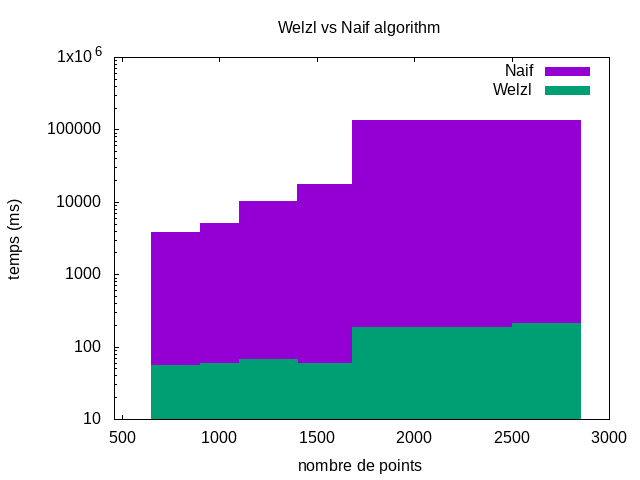
\includegraphics[width=370px,
                     keepaspectratio,]{welzlNaifPoints.png}\\
                     
    Ici aussi, nous remarquons que la forme des deux histogrammes se ressemblent mais que lorsque $n$ augmente, l'écart entre les 2 sommets de chaque algorithmes augmente de manière conséquente. Cela correspond donc bien au différences de complexité entre les deux algorithmes donc $O(n)$ pour l'algorithme de Welzl et $O(n^{4})$ pour le naïf.\\
\section{Conclusion}
    Nous avons constaté qu'en général, les deux algorithmes donnent des approximations du cercle minimum couvrant un ensemble de points fini, et donc que les cercles d'un même ensemble de points $P$ ne donnera pas forcément un cercle de diamètre égal. Cela est dû aux différences d'approches: quand l'algorithme naïf parcours les points de façon linéaire, l'algorithme de Welzl lui, parcours aléatoirement l'ensemble des points ce qui peut jouer sur la distance des points qu'il $compare^\eqref{eq:bases}$ et rends des cercles différents à chaque application de l'algorithme. Malgré les résultats aléatoires que donne l'algorithme de Welzl, la très grande majorité du temps il retourne un cercle se rapprochant du cercle minimum voir retourner le cercle minimum, ce qui est suffisant dans la majorité des cas en plus d'être très rapide avec une complexité temporelle linéaire. Un des problème rencontré avec l'algorithme de Welzl était dans l'implémentation, lorsque le plan contient beaucoup de points, la pile d'appels se remplit très vite et la machine ne pourra donc pas finir le calcul du cercle minimum, car elle ne pourra plus faire d'appel récursif au bout de $|Pile|$ récursion si la pile d'appels est rempli. Une solution possible serait de l'implémenter itérativement. 
    
    
    \newpage
    \begin{thebibliography}{}
    \bibitem{SED} Emo Welzl,
    \textit{Smallest enclosing disks (balls and ellipsoids).}
    Institut fiir Informatik, Freie Universi~t Berlin
    Amimallee 2-6, W 1000 Berlin 33, Germany\\
    \texttt{emo@tes.fu-berlin.de }
    \bibitem{Cours} Binh-Minh Bui-Xuan,
    \textit{Cours sur les collisions simples et problème du cercle minimum}\\
    \href{https://www-apr.lip6.fr/~buixuan/cpaad2020}{\texttt{https://www-apr.lip6.fr/~buixuan/cpaad2020}}
    \bibitem{Applications}
    \href{https://www.cs.mcgill.ca/~cs507/projects/1998/jacob/problem.html}{\texttt{https://www.cs.mcgill.ca/~cs507/projects/1998/jacob/problem.html}}
    \bibitem{bases}
    \href{http://www.sunshine2k.de/coding/java/Welzl/Welzl.html}{\texttt{http://www.sunshine2k.de/coding/java/Welzl/Welzl.html}}
    \bibitem{formules}
    \href{https://en.wikipedia.org/wiki/Smallest-circle\_problem}{\texttt{https://en.wikipedia.org/wiki/Smallest-circle\_problem}}
    \bibitem{tests} Base de tests de \textit{Varoumas}\\
    \href{http://www-apr.lip6.fr/~buixuan/files/cpaad2020/Varoumas_benchmark.zip}{http://www-apr.lip6.fr/~buixuan/files/cpaad2020/Varoumas\_benchmark.zip}
    \end{thebibliography}
\end{document}
